\documentclass[12pt]{article}
\usepackage[utf8]{inputenc}
\usepackage[margin=1in]{geometry}
\usepackage[spanish]{babel}\decimalpoint
\usepackage{setspace}\onehalfspacing
\usepackage{parskip} %Espacio entre parrafos.
\usepackage{graphicx} %Para usar \includegraphics[]{}
\usepackage{amssymb} %Para usar el si­mbolo del conj. de los Reales.%
\usepackage{amsmath} % Para usar columnas vectoriales.
\usepackage{multirow}
\usepackage{hyperref} %Siempre debe ser el ultimo paquete.


\setlength{\parindent}{0pt} %Texto justificado.
\setcounter{tocdepth}{2} %Que no incluya subsubsections en el índice.
%\setlength{\tabcolsep}{3pt}


%===================================================================%

\title{Apuntes `Calculus 1B: Integration'}
\author{}
\date{}

\begin{document}

\maketitle
\tableofcontents

\newpage

\section{La Integral.}

\subsection{Teorema del Valor Medio.}

En esta primera sección del curso, estudiaremos el Teorema del Valor Medio (\textit{Mean Value Theorem}). Veremos en qué consiste y cuándo se aplica.

También volveremos a revisar lo que nos dice el signo de una derivada (la primera) sobre el comportamiento de una función. Veremos que su \textbf{explicación} proviene (o es consecuencia) del teorema del valor medio. Durante este punto introduciremos los conceptos de \textbf{límite inferior} y \textbf{límite superior}.


\subsubsection{Vínculo entre la tasa de cambio promedio y la tasa de cambio instantánea.}

Imaginemos que hicimos un viaje en bus. Partimos en una ciudad A y llegamos a otra ciudad B. La distancia en ruta fue de 500 km y, sin que el vehículo se detuviera, demoramos 2 hrs en llegar hasta nuestro destino.

En ese sentido, si consideramos al tiempo que duró el viaje como $t$ hrs y a la distancia del recorrido en función del tiempo como $x(t)$ km, entonces podemos calcular que la rapidez promedio del bus fue:
\[
	\frac{x(2) - x(0)}{2 - 0} =
	\frac{500 - 0}{2 - 0} =
	250 \text{ km/hr}
\]
Si bien sabemos que la rapidez instantánea del bus puede haber variado con respecto a la promedio durante el trayecto, es posible suponer que en algún momento el vehículo alcanzó una rapidez de $250$ km/hr. En otras palabras, \textbf{es factible que en un tiempo $t = c$, la rapidez instantánea del bus sea igual a su rapidez promedio}. Esto puede ser explicado desde el Cálculo diferencial a partir del \textbf{Teorema de Valor Medio}.


\subsubsection{Teorema del Valor Medio.}

Sigamos con la función $x(t)$. El Teorema del Valor Medio (TVM, de ahora en adelante) indica que si se cumplen sus siguientes hipótesis:

\begin{itemize}
\item $x(t)$ es \textbf{continua} en un intervalo $a \leq t \leq b$.
\item $x(t)$ es \textbf{derivable} en un intervalo $a < t < b$.
\end{itemize}

Se puede concluir que:
\[
	\frac{x(b) - x(a)}{b - a} = x'(c) \qquad
	\text{para algún } c \text{ ubicado entre } a < c < b
\]
Aplicando un poco de álgebra, la conclusión del TVM también podemos escribirla de la siguiente forma:
\[
  x(b) = x(a) + x'(c)(b - a) \qquad \text{para algún } c \text{ ubicado entre } a < c < b
\]
Recordemos que la tasa de cambio promedio de una función, es la pendiente de una línea secante, mientras que en la tasa de cambio instantánea corresponde a la pendiente de su línea tangente. 

Al cumplirse las hipótesis del TVM en una función $x(t)$, su conclusión nos dice que la pendiente de la línea tangente en $(c, \ x(c))$ adentro de un intervalo $(a, \ b)$ \textbf{es paralela} a la pendiente de la línea secante entre los puntos $(a, \ x(a))$ y $(b, \ x(b))$, como lo vemos en la siguiente gráfica.

\begin{figure}[hbt!]
\centering
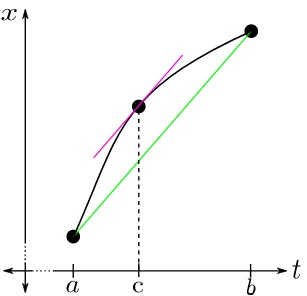
\includegraphics[scale=0.5]{img/mean-value-theo.jpg}
\end{figure}

El TVM no nos dice en cuál punto la pendiente de la línea tangente es igual a la de la línea secante, pero sí que podemos tener certeza que esto ocurrirá en algún valor $t = c$ en un intervalo $(a, \ b)$.

Otro aspecto a considerar es que, adentro del intervalo, \textbf{pueden existir más de una línea tangente con pendiente igual a la de la línea secante}.

\begin{figure}[hbt!]
\centering
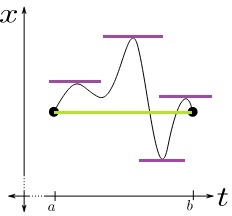
\includegraphics[scale=0.7]{img/mean-value-theo-2.jpg}
\end{figure}


\subsubsection{Cuándo sí falla el Teorema del Valor Medio y cuándo no.}

El TVM no siempre se aplicará a todas las funciones o a todos los intervalos. Fundamentalmente, \textbf{fracasará cuando su conclusión nunca se cumpla adentro del intervalo de interés}.

Por ejemplo, veamos las siguientes gráficas.

\begin{figure}[hbt!]
\centering
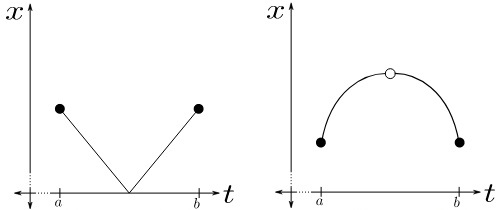
\includegraphics[scale=0.6]{img/mean-value-theo-3.jpg}
\end{figure}

Como se puede apreciar, en ambas gráficas es posible trazar una línea secante entre los puntos $(a, \ x(a))$ y $(b, \ x(b))$. Sin embargo, donde la pendiente de una línea tangente podría ser igual a la misma de la línea secante, en el gráfico izquierdo, ésta no existe y en el del lado derecho, hay una discontinuidad y, por tanto, tampoco es posible calcular la derivada en dicho lugar. Por lo tanto, \textbf{el TVM falla en aplicarse} porque \textbf{no se cumple su conclusión}.

Veamos ahora el siguiente gráfico.

\begin{figure}[hbt!]
\centering
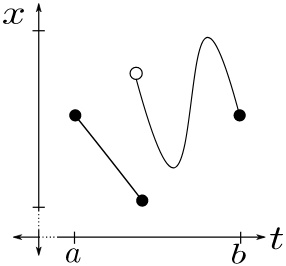
\includegraphics[scale=0.5]{img/mean-value-theo-4.jpg}
\end{figure}

Si nos damos cuenta, en el gráfico de arriba podemos trazar una línea secante adentro del intervalo $[a, \ b]$ y su pendiente puede ser igual a la de algunas líneas tangentes que es posible encontrar en $(a, \ b)$. Sin embargo, $x(t)$ no es continua en $[a, \ b]$.

\begin{figure}[hbt!]
\centering
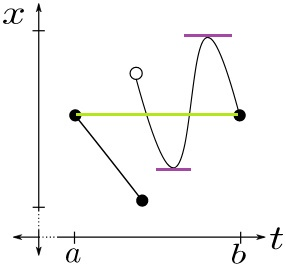
\includegraphics[scale=0.5]{img/mean-value-theo-5.jpg}
\end{figure}

¿El TVM se contradice en este caso? \textbf{No, porque la conclusión de un teorema puede ser satisfecho incluso si no lo hacen sus hipótesis}.

\newpage

\subsubsection{El TVM y el comportamiento de una función según el signo de su derivada.}

Digamos que tenemos dos números $a$ y $b$ tal que $b > a$. Probablemente recordaremos que:

\begin{itemize}
\item Si $f(b) \geq f(a)$ entonces $f(x)$ está \textbf{creciendo}.
\item Si $f(b) \leq f(a)$ entonces $f(x)$ está \textbf{decreciendo}.
\end{itemize}

Y cuando estudiamos sobre derivadas al inicio, aprendimos que:

\begin{itemize}
\item Si $f'(x) > 0$ entonces $f(x)$ está \textbf{creciendo}.
\item Si $f'(x) < 0$ entonces $f(x)$ está \textbf{decreciendo}.
\item Si $f'(x) = 0$ entonces $f(x)$ es \textbf{constante}.
\end{itemize}

El vínculo entre el signo de la derivada de una función y su comportamiento, lo sabemos intuitivamente. Ahora veremos que, a partir del Teorema del Valor Medio, podemos darle una explicación a ese hecho.

Para explicar lo anterior, usemos las nociones de los \textbf{límites inferior y superior}\footnote{En inglés corresponden a \textit{lower bound} y \textit{upper bound}, por tanto asumo que también pueden traducirse como ``cota inferior'' y ``cota superior'', respectivamente.}.

El \textbf{límite inferior} en una función es un número que es menor o igual a todos los valores que ésta puede tomar. Mientras que el \textbf{límite superior} es un valor que es mayor o igual a todos los \textit{output} de una función.

En otras palabras:

\begin{itemize}
\item Un número $m$ es un \textbf{límite inferior} de $f(x)$ si $m \leq f(x)$ para todo $x$.
\item Un número $M$ es un \textbf{límite superior} de $f(x)$ si $M \geq f(x)$ para todo $x$.
\end{itemize}

Por lo tanto, para todos los $\mathbb{R}$ o adentro de un intervalo, se puede concluir que:
\[
  m \leq f(x) \leq M
\]
Veamos como ejemplo el siguiente gráfico, donde $y = f(x)$.

\newpage

\begin{figure}[hbt!]
\centering
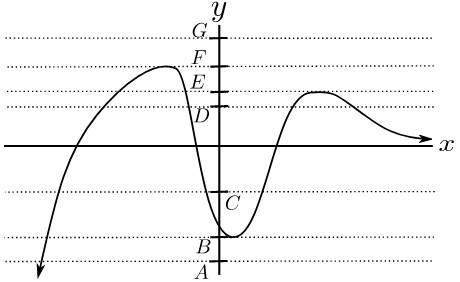
\includegraphics[scale=0.6]{img/bounds-mvt.jpg}
\end{figure}

Para todo $x \in \mathbb{R}$, entre los números $A, \ B, \ C, \ 0, \ E, \ F$ y $G$, la función $f(x)$ no tiene un límite inferior, pero sí tiene límites superiores, los cuales son $F$ y $G$ puesto que son mayores o iguales a esta función.

Pero ahora busquemos estos límites adentro de un intervalo $[a, \ b]$.

\begin{figure}[hbt!]
\centering
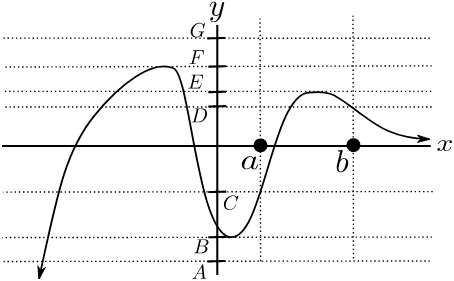
\includegraphics[scale=0.6]{img/bounds-mvt-2.jpg}
\end{figure}

En este caso podemos decir que, para todo $x \in [a, \ b]$, $f(x)$ tiene tanto límites inferiores como superiores:

\begin{itemize}
\item Límites inferiores: $A, \ B, \ C$.
\item Límites superiores: $E, \ F, \ G$.
\end{itemize}

Entonces, en un intervalo cerrado es más fácil asegurar que una función tendrá al menos un límite inferior y uno superior que cuando uno o ambos están abiertos, o a lo largo de la recta de los $\mathbb{R}$.

Si queremos tener más precisión sobre la ubicación de $f(x)$, podemos buscar el \textbf{límite superior mínimo} (i.e, el límite superior más chico) y/o \textbf{límite inferior mayor} (i.e, el límite inferior más grande).

En ese sentido, a partir del último gráfico de $f(x)$ que vimos y adentro de $[a, \ b]$, es posible decir que su límite inferior mayor es $C$, mientras que su límite superior mínimo es $E$.

Usemos ahora las nociones de los límites inferior y superior, así como lo planteado en el teorema del valor medio, para que el signo de la derivada de una función nos indica el comportamiento de ésta.

Sea $x(t)$ una función continua en $[A, \ B]$ y derivable en $(A, \ B)$. Según el TVM, podemos garantizar que:
\[
  \frac{x(B) - x(A)}{B - A} = x'(c) \qquad \text{para algún } c \text{ en } (A, \ B)
\]
Digamos que $m$ es un \textbf{límite inferior} de $x'(t)$. Esto implica que:
\[
  m \leq x'(t) \qquad \forall t \in (A, \ B)
\]
Basándonos en el TVM, podemos establecer que $m$ también es un límite inferior de la tasa de cambio promedio de $x(t)$ entre $[A, \ B]$.
\[
  m \leq \frac{x(B) - x(A)}{B - A}
\]
Si $m$ es un límite inferior de $x'(t)$ en $(A, \ B)$, también puede serlo en un intervalo más chico $(a, \ b)$ que está adentro del antes señalado. Por lo tanto:
\[
  m \leq x'(t) \qquad \forall \ a, b \text{ entre } A \leq a < b \leq B
\]
En consecuencia, por medio del TVM, $m$ no solo es un límite inferior de la tasa de cambio promedio entre $[A, \ B]$, sino que también en el intervalo más chico $[a, \ b]$ que se encuentra adentro de $[A, \ B]$.
\[
  m \leq \frac{x(b) - x(a)}{b - a} \qquad \forall \ a, b \text{ entre } A \leq a < b \leq B
\]
Sigamos en el intervalo $(a, \ b) \subseteq (A, \ B)$, pero ahora definamos que $m = 0$ es el límite inferior de $x'(t)$. A partir de lo anterior, sabemos que:
%
%\newpage
%
%Si esto aún no nos está dando un atisbo sobre el comportamiento de una función según el valor de su derivada, entonces digamos que $m = 0$ es un límite inferior de $x'(t)$.
\[
  0 \leq x'(t) \qquad \forall \ a, b \text{ entre } A \leq a < b \leq B
\]
Y que, por el TVM, entonces:
\[
  0 \leq \frac{x(b) - x(a)}{b - a} \qquad \forall \ a, b \text{ entre } A \leq a < b \leq B
\]
Si esta desigualdad la multiplicamos por $(b - a)$ y la sumamos por $x(a)$, obtenemos que:
\[
  x(a) \leq x(b)
\]
Es decir, cuando $x'(t) \geq 0$ para todo $t$ en $A \leq a < b \leq B$, la función $x(t)$ está creciendo o manteniéndose estable (i.e, constante) en $[a, \ b]$ y, por consiguiente, en $[A, \ B]$, como consecuencia del TVM.

Ahora digamos que $m = 0$ es el \textbf{límite superior} de $x'(t)$ en $(a, \ b) \subseteq (A, \ B)$. Esto significa que:
\[
  0 \geq x'(t) \qquad \forall \ a, b \text{ entre } A \leq a < b \leq B
\]
Y, debido al TVM, entonces:
\begin{align*}
0 &\geq \frac{x(b) - x(a)}{b - a} \qquad \forall \ a, b \text{ entre } A \leq a < b \leq B \\
x(a) &\geq x(b)
\end{align*}
Cuando $x'(t) \leq 0$ para todo $t$ en $(a, b) \subseteq [A, \ B]$, $x(t)$ está decreciendo o manteniéndose constante en $[a, \ b]$ y en $[A, \ B]$.

Entonces, como consecuencia del Teorema del Valor Medio, podemos concluir que si:

\begin{itemize}
\item $x'(t) > 0$ $\forall t \in (A, \ B)$ entonces $x(t)$ está \textbf{creciendo} a lo largo de $[A, \ B]$.
\item $x'(t) < 0$  $\forall t \in (A, \ B)$ entonces $x(t)$ está \textbf{decreciendo} a lo largo de $[A, \ B]$.
\item $x'(t) = 0$  $\forall t \in (A, \ B)$ entonces $x(t)$ es \textbf{constante} a lo largo de $[A, \ B]$.
\end{itemize}

\textbf{Ejercicio.} \quad En cada momento durante el mes de julio, un incendio está creciendo a una tasa de, al menos, $2 \text{ km}^{2}$ por día.

Si para el 15 de julio, el área del incendio es de $50 \text{ km}^{2}$, ¿cuál será su medida para el 25 y para el 5 del mismo mes?

\textbf{Solución.} \quad Definamos el área del incendio en función del tiempo como $A_{I}(t)$, el cual es medido en $\text{km}^{2}$.

Como el incendio está creciendo durante todo julio, es válido asumir que $A_{I}(t)$ es continua y derivable en todos los días del mes. Por lo tanto, a partir del TVM podemos asegurar que al menos en uno de esos días, la tasa de crecimiento promedio del área en todo el mes será igual a la tasa de crecimiento del mismo en dicho día.

%Debido a que el incendio está creciendo durante todo el mes de julio (i.e, sin parar), la función $A_{I}(t)$ debería ser continua entre los días $[1, \ 31]$ y también derivable en $(1, \ 31)$. Por lo tanto, si nos basamos en el TVM, podemos asegurar que la tasa de crecimiento del área del incendio en al menos un día va a ser igual a la tasa de crecimiento promedio en todo el mes del mismo.

En el ejercicio nos dicen que el límite superior mínimo de $A'_{I}(t)$, es $2 \text{ km}^{2}$ en cada día de julio.
\[
  2 \text{ km}^{2} / \text{ día} \geq A'_{I}(t) \qquad \forall t \in (1, \ 31) \text{ días}
\]
El límite superior mínimo de $A'_{I}(t)$ puede serlo tanto para todo el mes como para un intervalo de días adentro del mismo período. Tener en cuenta aquello nos sirve bastante, porque nos piden calcular el área que tendrá el incendio el día 25 y el que tuvo el día 5, sabiendo que para el día 15 midió $50 \text{ km}^{2}$. Entonces, lo que podemos hacer es asumir que dicho límite lo es para los días $(15, \ 25)$ como para los días $(5, \ 15)$ y aplicar el TVM en ambos casos.

Para el intervalo $(15, \ 25)$ tenemos que:
\begin{align*}
\frac{A_{I}(25) - 50}{25 - 15} \text{ km}^{2}/ \text{ día} &\leq 2 \text{ km}^{2}/ \text{ día} \\
A_{I}(25) &\leq 70 \text{ km}^{2}
\end{align*}
Y para el intervalo $(5, \ 15)$:
\begin{align*}
\frac{50 - A_{I}(5)}{15 - 5} \text{ km}^{2}/ \text{ día} &\leq 2 \text{ km}^{2}/ \text{ día} \\
A_{I}(5) &\geq 30 \text{ km}^{2}
\end{align*}
Entonces, podemos concluir que para el día 15 de julio, el área del incendio es al menos de 70 $\text{km}^{2}$, mientras que para el 5 de julio es de, a lo más, 30 $\text{km}^{2}$.

\textbf{Ejercicio 2.} \quad Demuestre que $e^{x} > 1 + x$, para todo $x > 0$.

\textbf{Solución} \quad Podemos partir definiendo la siguiente función:
\[
  h(x) = e^{x} - (1 + x)
\]
Un primer hecho que podemos constatar es que si $x = 0$, entonces $h(0) = 0$.

Ahora, derivemos $h(x)$.
\[
  h'(x) = e^{x} - 1
\]
Si observamos bien, para todo $x > 0$, $h'(x)$ siempre se mantendrá creciendo. Es decir, $h'(x) > 0$ para todo $x > 0$ y, como consecuencia del TVM, podemos afirmar que $h(x)$ está creciendo en dicho intervalo. Por lo tanto, es verdadero que:
\[
  h(x) > h(0) \qquad \forall x > 0
\]
Reemplacemos $h(x)$ y $h(0)$ en aquella desigualdad:
\[
  e^{x} - (1 + x) > 0 \qquad \forall x > 0 
\]
Si despejamos $e^{x}$, obtenemos que:
\[
  e^{x} > 1 + x \qquad \forall x > 0
\]
Quedando así demostrada aquella afirmación.

\subsubsection{Acotando (\textit{bounding}) la tasa de cambio promedio.}

Cuando hacemos un viaje en vehículo desde un lado a otro, podemos asegurar intuitivamente que la rapidez promedio se encontrará entre la rapidez mínima y máxima que alcance en un momento u otro del trayecto. La justificación de este hecho la podemos encontrar, desde la matemática, en el TVM.

Sea $x(t)$ una función continua en $[a, \ b]$ y derivable en $(a, \ b)$. Como ya sabemos, dadas estas características podemos asegurar, a partir del TVM, que:
\[
  \frac{x(b) - x(a)}{b - a} = x'(c) \qquad \text{para algún } c \text{ en } a < c < b
\]
Digamos que ese $x'(c)$ tiene un límite inferior $m$ y un límite superior $M$. En otras palabras:
\[
  m \leq x'(c) \leq M \qquad \forall c \in (a, \ b)
\]
Por el TVM, lo anterior implica que:
\[
  m \leq \frac{x(b) - x(a)}{b - a} \leq M
\]
Ahora, supongamos que conocemos el valor mínimo y máximo que alcanza $x'(t)$ en $(a, \ b)$. Dichos valores podemos entenderlos como el límite inferior mayor y el límite superior mínimo de aquella derivada, respectivamente\footnote{Buscamos los valores máximo y mínimo en un intervalo cerrado puesto que, según el Teorema del Valor Extremo, cuando una función es continua en ese lugar, podemos garantizar la existencia de ambos adentro de ese rango de valores.}.
\[
  \min_{a \leq c \leq b} x'(t) \leq x'(c) \leq \max_{a \leq c \leq b} x'(t)
\]

\newpage

Y, nuevamente, por el TVM podemos establecer que
\[
  \min_{a \leq c \leq b} x'(t) \leq \frac{x(b) - x(a)}{b - a} \leq \max_{a \leq c \leq b} x'(t)
\]
Si $x(t)$ fuese la distancia que toma el vehículo en función del tiempo y $x'(t)$ su rapidez en cada momento $t$, entonces a partir de la desigualdad de arriba hemos justificado que, efectivamente, su rapidez promedio del trayecto puede estar entre la rapidez mínima y la rapidez máxima que alcanzó en algún momento del viaje.

Por otra parte, el $\min_{a \leq c \leq b} x'(t)$ y el $\max_{a \leq c \leq b} x'(t)$ son los mejores límites inferior y superior de $x'(t)$, entonces también podemos precisar que
\[
  m \leq \min_{a \leq c \leq b} x'(t) \leq x'(t) \leq \max_{a \leq c \leq b} x'(t) \leq M
\]
Y, por tanto, a partir del TVM lo anterior implica que:
\[
  m \leq \min_{a \leq c \leq b} x'(t) \leq \frac{x(b) - x(a)}{b - a} \leq \max_{a \leq c \leq b} x'(t) \leq M
\]
\textbf{Ejercicio 3.} \quad Encuentre la constante $C$ más pequeña tal que
\[
  \lvert \sin(b) - \sin(a) \rvert \leq C \lvert b - a \rvert \qquad \text{para cualquier } a, \ b
\]
\textbf{Solución.} \quad Primero, asumamos que $a < b$.

Como el $\sin(t)$ es continua y derivable en todos los $\mathbb{R}$, también lo será para un intervalo $[a, \ b]$. Por lo tanto, podemos asegurar a partir del TVM que:
\begin{align*}
  \frac{\sin(b) - \sin(a)}{b - a} &= \sin'(c) \\
  \frac{\sin(b) - \sin(a)}{b - a} &= \cos(c) \qquad \text{para algún } c \text{ en } a < c < b
\end{align*}
El $\cos(t)$ es continua en todos los $\mathbb{R}$ y, por tanto, también en $[a, \ b]$, de manera que podemos garantizar a partir del Teorema del Valor Extremo que su valor máximo y mínimo se encuentran en dicho intervalo.
\[
  \min_{a \leq t \leq b} \cos(t) \leq
  \cos(t) \leq
  \max_{a \leq t \leq b} \cos(t) \qquad
  \forall t \in (a, \ b)
\]
Y, por el TVM, entonces:
\[
  \min_{a \leq t \leq b} \cos(t) \leq
  \frac{\sin(b) - \sin(a)}{b - a} \leq
  \max_{a \leq t \leq b} \cos(t) \qquad
  \text{para cualquier } a < b
\]
Ahora, un problema con esta desigualdad es que los valores máximo y mínimo de $\cos(t)$ son aquellos que están adentro del $[a, \ b]$ y, en realidad, es más de nuestro interés que sean dichos valores pero para todos los de ese intervalo. Por lo tanto, definámoslos para todos los $\mathbb{R}$:
\[
  \min_{-\infty < t < \infty} \cos(t) \leq
  \frac{\sin(b) - \sin(a)}{b - a} \leq
  \max_{-\infty < t < \infty} \cos(t) \qquad
  \text{para cualquier } a < b
\]
Y los máximo y mínimo global que puede tomar el $\cos(t)$ en los $\mathbb{R}$, son $1$ y $-1$.
\[
  -1 \leq \frac{\sin(b) - \sin(a)}{b - a} \leq 1
\]
Podemos demostrar lo anterior calculando la derivada del $\sin(t)$ en $t = 0$ y $t = \pi$ usando la definición de la misma, para cualquier $a < b$:
\begin{align*}
  \sin'(0) &= \lim_{b \to 0} \frac{\sin(b) - \sin(0)}{b - 0} &
  \sin'(\pi) &= \lim_{b \to \pi} \frac{\sin(b) - \sin(\pi)}{b - \pi} \\
  \sin'(0) &= -1 &
  \sin'(\pi) &= 1
\end{align*}
Recordemos que la expresión que intentamos demostrar, usa valores absolutos. Si calculamos el valor absoluto de la desigualdad de arriba, obtendremos que:
\[
  \left\lvert \frac{\sin(b) - \sin(a)}{b - a} \right\rvert \leq 1 \qquad \text{para cualquier } b < a
\]
Pero el lado izquierdo también corresponde a:
\[
  \frac{\sin(b) - \sin(a)}{b - a} = \frac{\sin(a) - \sin(b)}{a - b}
\]
Donde:
\[
  \left\lvert \frac{\sin(a) - \sin(b)}{a - b} \right\rvert \leq 1 \qquad \text{para cualquier } a < b
\]
Y si señalamos que $a > b$, entonces:
\[
  \left\lvert \frac{\sin(b) - \sin(a)}{b - a} \right\rvert \leq 1 \qquad \text{para cualquier } a > b
\]
En otras palabras, es válido señalar que:
\[
  \left\lvert \frac{\sin(b) - \sin(a)}{b - a} \right\rvert \leq 1 \qquad \text{para cualquier } a, \ b
\]
Por consiguiente, si a la desigualdad la multiplicamos por $(b - a)$, entonces:
\[
  \left\lvert \sin(b) - \sin(a) \right\rvert \leq 1 \cdot (b - a) \qquad \text{para cualquier } a, \ b
\]
Es decir, $C = 1$ es la constante más pequeña de la desigualdad de arriba, para cualquier $a$ y $b$.


\subsubsection{Comparación entre la Aproximación Lineal y el TVM.}

Quizá hemos notado cierta similitud entre lo que indica el TVM y el cálculo de la aproximación lineal de una función. Ambas se asemejan en que, con ellas, podemos obtener información sobre \textbf{el cambio de una función en un intervalo}, pero sus declaraciones y propósitos son distintos.

La idea de la aproximación lineal es estimar el valor de una función, calculando la pendiente de una línea tangente bastante cercano a éste. En otras palabras, se intenta aproximar una función general por medio de una función lineal.

Por ejemplo, digamos que queremos conocer el valor de una función $x(t)$. Aquello podemos lograrlo, calculando su derivada en $t \approx a$.
\begin{align*}
  \frac{x(t) - x(a)}{t - a} &\approx x'(a) \\
  x(t) &\approx x(a) + x'(a)(t - a)
\end{align*}
Mientras que, como ya lo hemos estudiado, el TVM concluye que si una función $x(t)$ es continua en $[a, \ b]$ y derivable en $(a, \ b)$, podemos asegurar que en algún punto $t = c$ entre $a < c < b$, la derivada en ese lugar será igual a la pendiente de la línea secante entre $[a, \ b]$.
\[
  \frac{x(b) - x(a)}{b - a} = x'(c) \qquad \forall c \in (a, \ b)
\]
Como vemos, a partir del TVM se asegura que habrá una igualdad entre la pendiente de una línea secante y la pendiente de una línea tangente entre los puntos de la primera, aunque no sabemos en qué punto en particular. En cambio, en la aproximación lineal nos acercamos a un valor, pero a partir de un punto que elegimos, por lo que estamos en conocimiento de éste.

Para terminar, en la siguiente imagen tenemos la comparación geométrica de la aproximación lineal y del TVM que nos sirve para ilustrar los mencionado anteriormente.

\begin{figure}[hbt!]
\centering
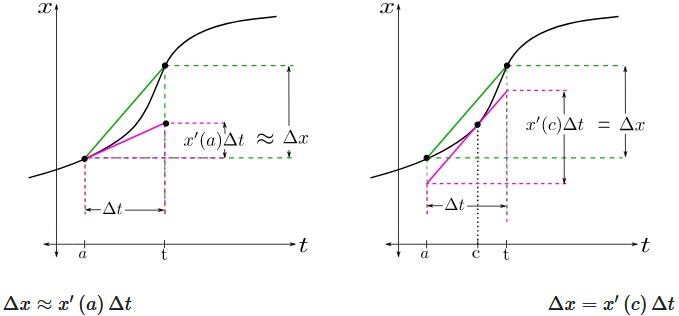
\includegraphics[scale=0.5]{img/mean-value-theo-linear-approx.jpg}
\end{figure}



\subsection{Diferenciales y Antiderivadas.}

Desde esta sección comenzaremos a introducirnos en el tema central de este curso: las integrales. Para ello, nos centraremos en dos conceptos, el de los diferenciales y el de las antiderivadas o integrales infinitesimales.

Veremos que el \textbf{diferencial} es la interpretación que le da Leibniz a la derivada, entendiéndola como una proporción entre el cambio en $y$ y el cambio en $x$. También buscaremos la \textbf{antiderivada} de una función, la cual corresponde a una derivada y vamos a buscar las funciones que nos permitan obtenerla. En otras palabras, realizaremos el cálculo inverso de la derivada.


\subsubsection{Diferenciales.}

Digamos que $y = f(x)$, con $y$ dependiendo de $x$. Sabemos que la derivada de esta función corresponde a:
\[
  f'(x) = \lim_{\Delta x \to 0} \frac{\Delta y}{\Delta x}
        = \lim_{\Delta x \to 0} \frac{f(x + \Delta x) - f(x)}{\Delta x}
\]
Leibniz intuitivamente interpretó la derivada como \textbf{el cuociente entre los cambios infinitesimales de $y$ y de $x$}, denotándola como:
\[
  \frac{dy}{dx} = f'(x)
\]
Las expresiones $dy$ y $dx$ corresponden a los \textbf{diferenciales} de $y$ y de $x$. Si bien ambos representan cambios infinitamente pequeños de las dos variables, aún así conllevan a una proporción que es expresada por $f'(x)$ y cuya medición no es tan chica.

Si consideramos a $dy$ y a $dx$ como cantidades, es posible establecer que:
\[
  dy = f'(x)dx
\]
La utilidad que tienen los diferenciales, es que nos permiten hacer un seguimiento del cambio de $y$ cuando $x$ lo hace por una cantidad muy pequeña. Por ejemplo, si queremos saber cómo va cambiando una distancia $x(t)$ km en cada tiempo $t$ hr, lo calculamos como:
\[
  d(x(t)) = x'(t) \cdot dt
\]
Donde $d(x(t))$ se mide en km, $x'(t)$ en km/hr y $dt$ en hr.

\textbf{Ejercicio.} \quad Sea $f(w) = 3w^{-1} + w^{2}/4 - 7$, calcule el diferencial de $f(w)$.

\textbf{Solución.} \quad Si usamos la última igualdad de arriba, podemos expresar el diferencial de $f(w)$ como:
\begin{align*}
  d(f(w)) &= f'(w) dw \\
  d\left(3w^{-1} + \frac{w^{2}}{4} - 7\right) &= \left(-3w^{-2} + \frac{1}{2}w\right) dw
\end{align*}
\textbf{Ejercicio 2.} \quad Calcule el diferencial de $\ln(y^{2}) + \ln(1 + \sqrt{y})$.

\textbf{Solución.} \quad Al igual que en el ejercicio anterior, usamos la fórmula que nos da el diferencial de una función.
\begin{align*}
  d(\ln(y^{2}) + \ln(1 + \sqrt{y})) &= \left(
                                          \frac{1}{y^{2}} \cdot 2y +
                                          \frac{1}{1+\sqrt{y}} \cdot \frac{1}{2\sqrt{y}}
                                        \right) dy \\
                                    &= \left(\frac{2}{y} + \frac{1}{2\sqrt{y}(1 + \sqrt{y})}\right) dy
\end{align*}

\subsubsection{Cálculo de la Aproximación Lineal usando Diferenciales.}

Como sabemos, la aproximación lineal es un método para estimar el valor de una función, usando su derivada. Ahora veremos que, a partir de su explicación geométrica, también podemos entender desde esta perspectiva a los diferenciales y usarlos para calcular de otra forma esta aproximación.

Digamos que $y = f(x)$ y queremos estimar un valor de ella a partir de su aproximación lineal cerca de $x = x_{0}$. Como se aprecia en el siguiente gráfico, lo que hacemos es trazar una línea tangente en el punto $(x_{0}, \ f(x_{0}))$, con pendiente igual a $f'(x_{0})$ y cuya función (también llamada la linealización de $f(x)$) es $L(x)$:

\begin{figure}[hbt!]
\centering
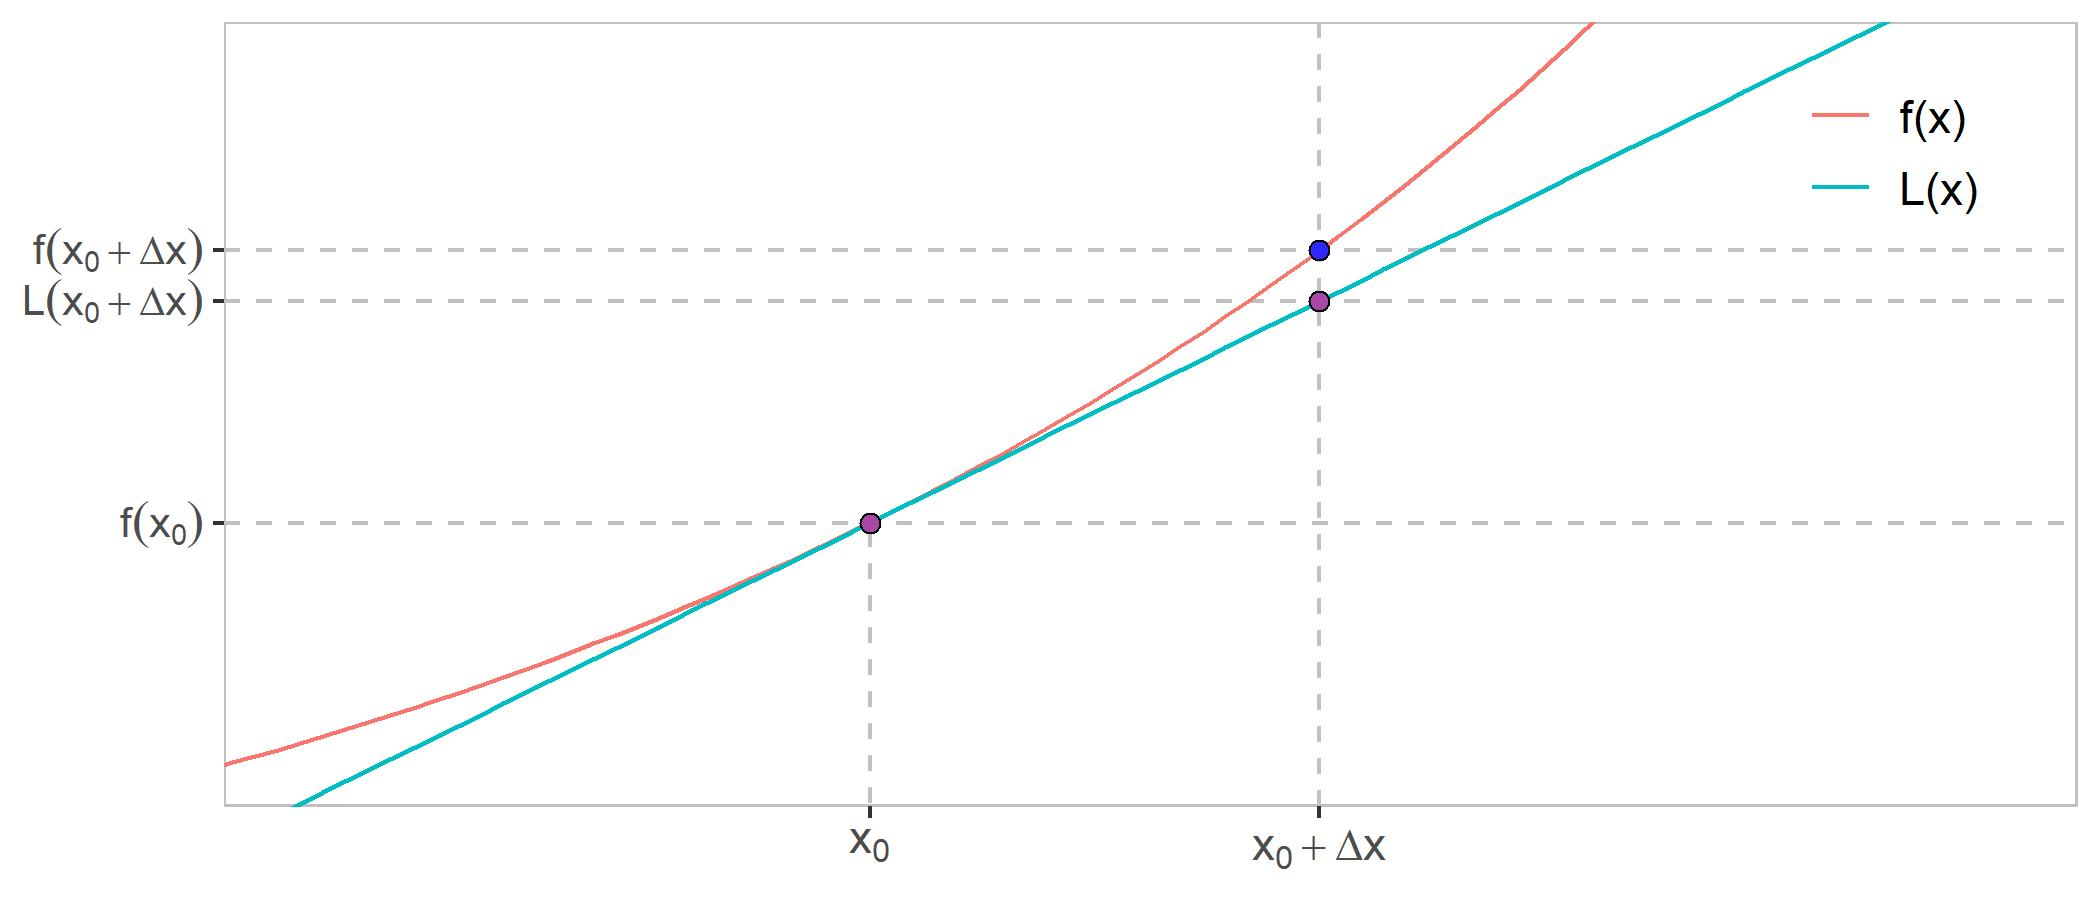
\includegraphics[scale=0.7]{img/diff_examp_plot.jpg}
\end{figure}

Donde $L(x) = f(x_{0}) + f'(x_{0})(x - x_{0})$ y $L(x) \approx f(x)$ para todo $x$.

La idea es ver a qué valor se aproxima $f(x)$ cuando $x = x_{0} + \Delta x$, lo cual evaluamos a partir de $L(x)$ en el mismo punto. Es decir, $f(x_{0} + \Delta x) \approx L(x_{0} + \Delta x)$. Si reemplazamos con la función dada por $L(x)$, entonces:
\begin{align*}
  f(x_{0} + \Delta x) &\approx L(x_{0} + \Delta x) = f(x_{0}) + f'(x_{0})((x_{0} + \Delta x) - x_{0}) \\
                      &\approx L(x_{0} + \Delta x) = f(x_{0}) + f'(x_{0}) \Delta x
\end{align*}
Fijémonos ahora qué ocurre cuando restamos la expresión de arriba por $f(x_{0})$.
\[
  f(x_{0} + \Delta x) - f(x_{0}) \approx L(x_{0} + \Delta x) - f(x_{0}) = f'(x_{0}) \Delta x
\]
Al observar bien, nos daremos cuenta que $\Delta f = f(x_{0} + \Delta x) - f(x_{0})$ y $\Delta L = L(x_{0} + \Delta x) - f(x_{0})$. Es decir, y como vemos en la siguiente figura, corresponden a las mediciones de los cambios de $f(x)$ y $L(x)$ a lo largo de sus gráficas a medida que $x$ se mueve desde $x_{0}$ hasta $x_{0} + \Delta x$.

\begin{figure}[hbt!]
\centering
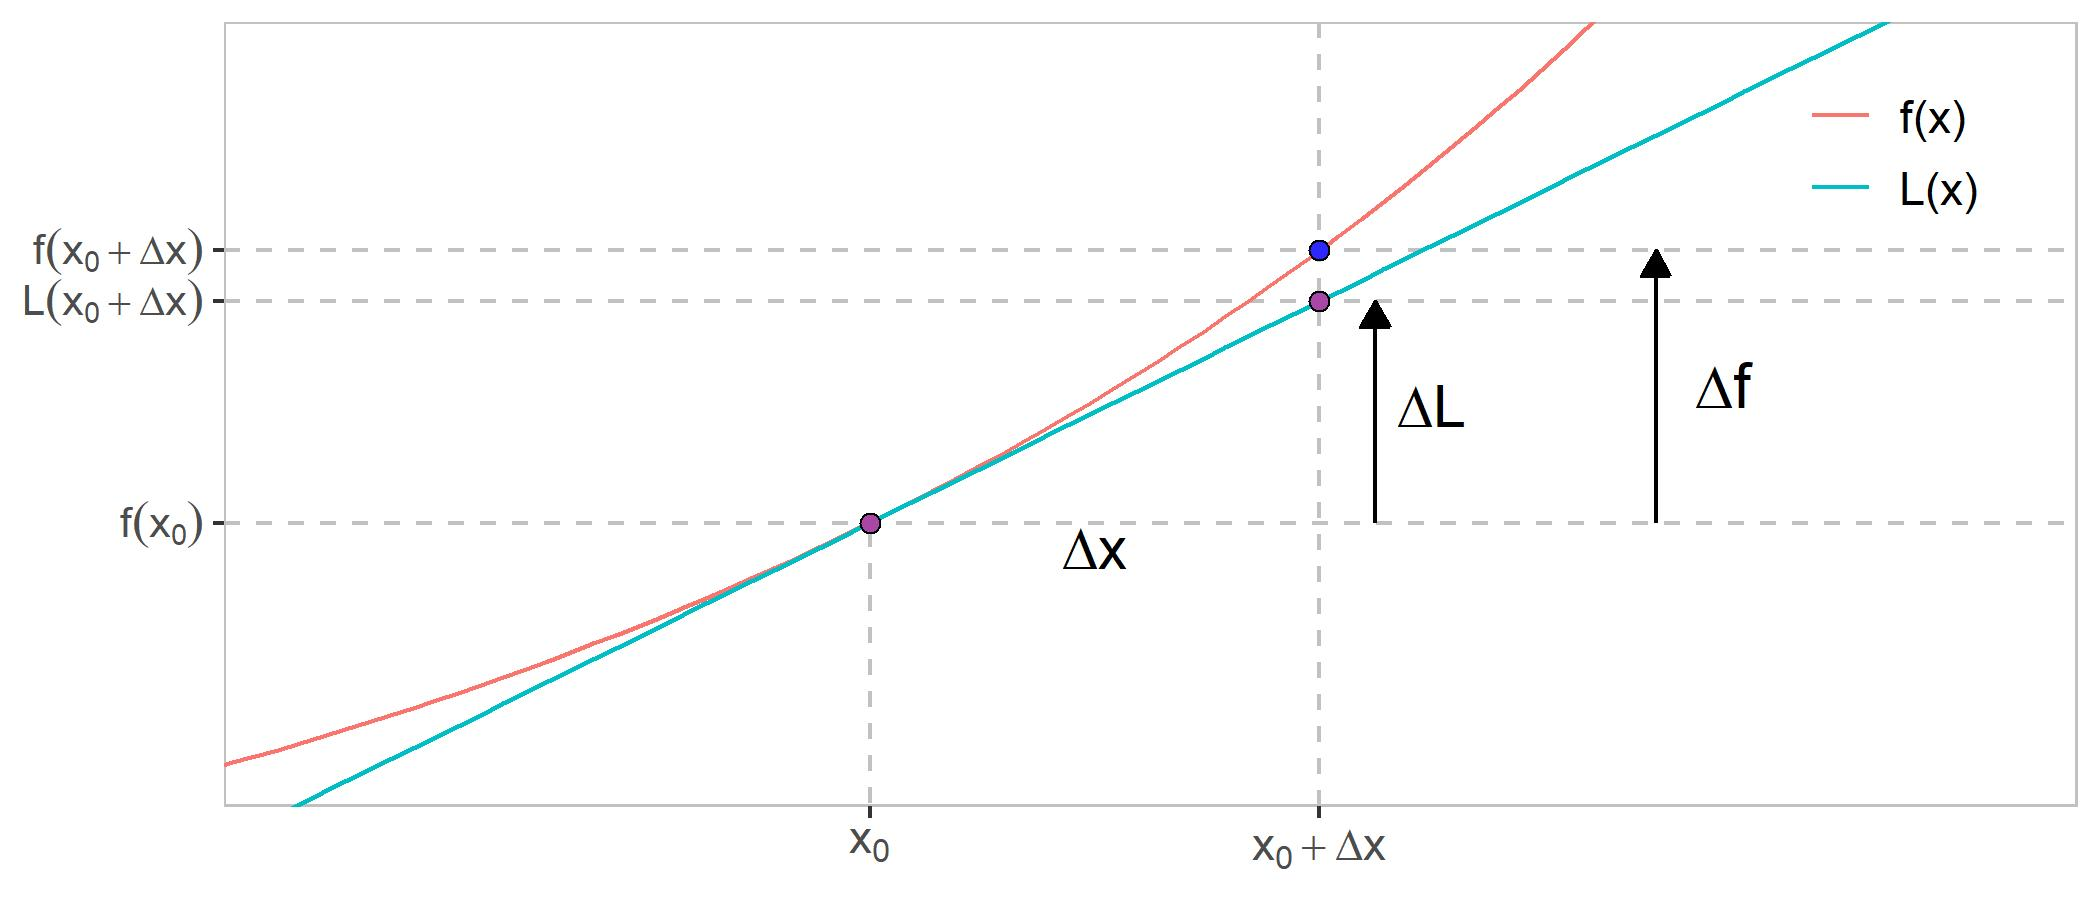
\includegraphics[scale=0.7]{img/diff_examp_plot_2.jpg}
\end{figure}

Por lo tanto, podemos establecer que:
\[
  \Delta f \approx \Delta L = f'(x_{0}) \Delta x
\]
La medida $\Delta f$ es el cambio exacto de $f(x)$ en la distancia $\Delta x$ y $\Delta L$ también lo es, pero de la línea tangente $L(x)$, por lo tanto es una aproximación (lineal) a $\Delta f$.

Si usamos la interpretación de Leibniz de la derivada, entonces nos percataremos que este cambio a lo largo de la línea tangente, corresponde al diferencial de la función principal $f(x)$. Es decir, $\Delta L = df$. Y éste depende del cambio en $x$, de manera que $dx = \Delta x$. Por lo tanto:
\[
  \Delta f \approx df = f'(x_{0}) dx
\]
Modifiquemos el anterior gráfico con lo que acabamos de aprender.

\begin{figure}[hbt!]
\centering
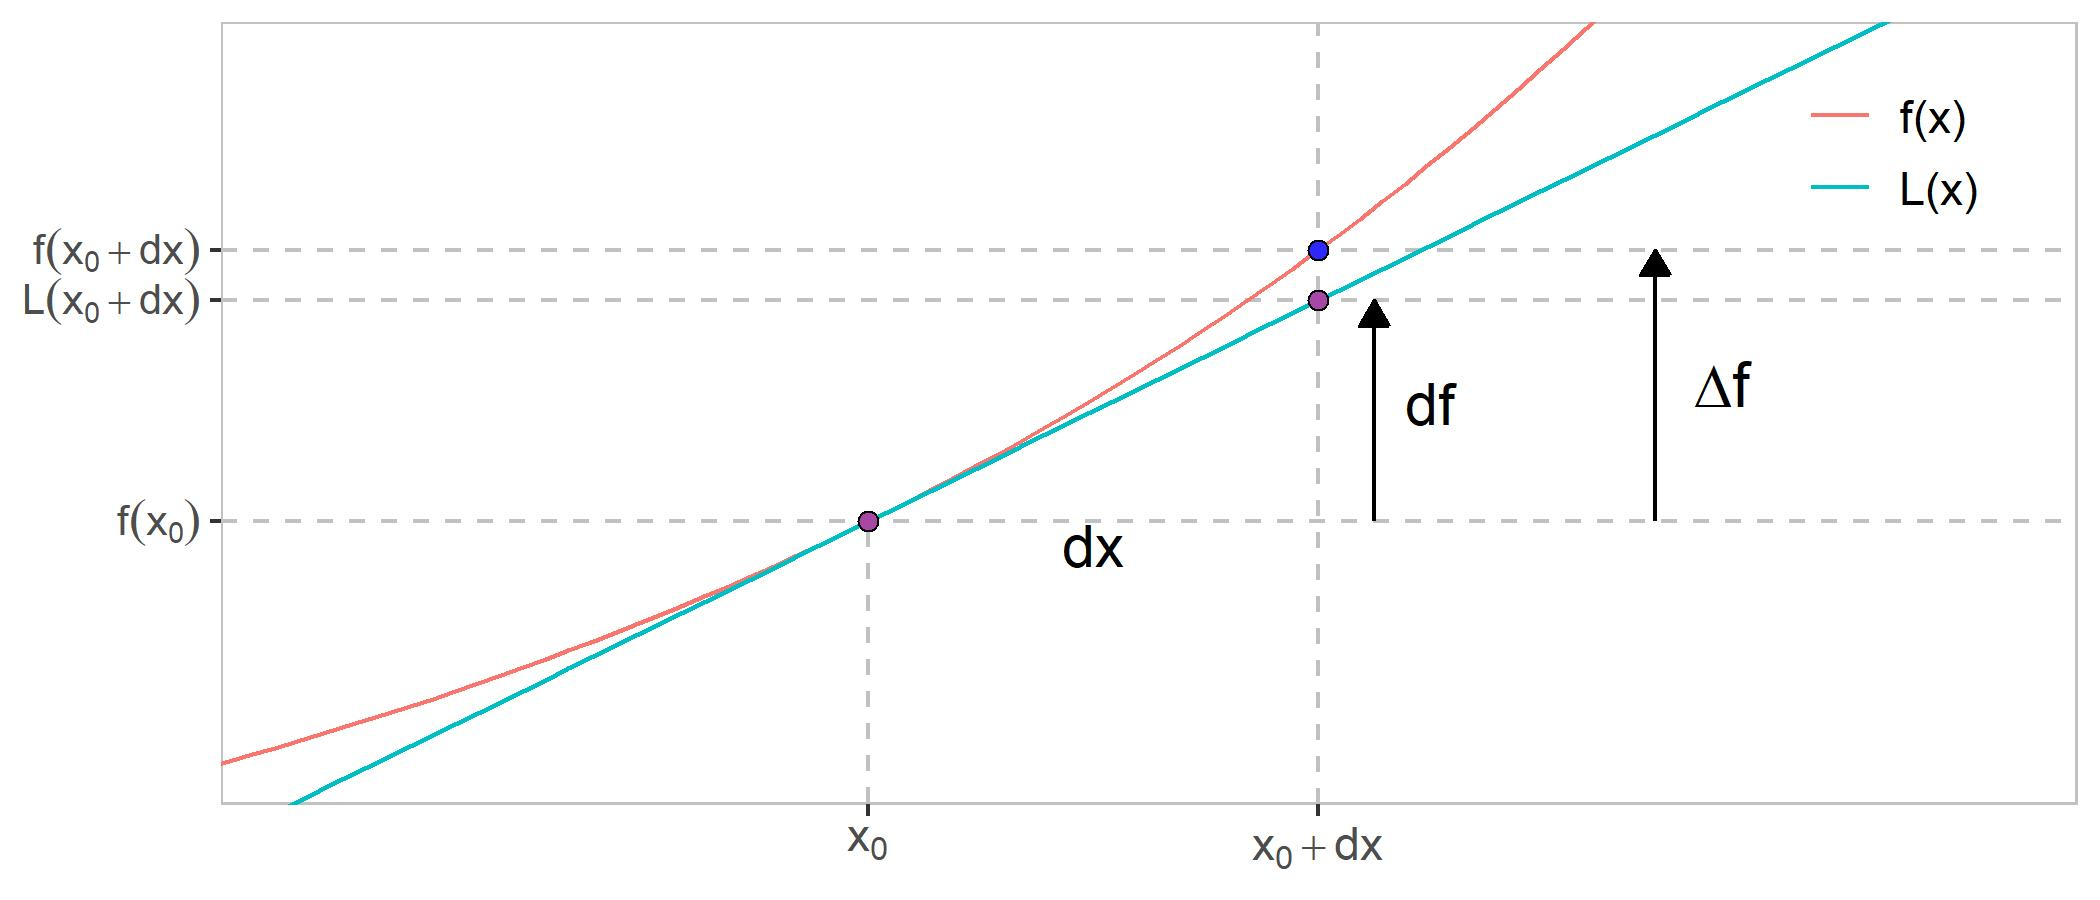
\includegraphics[scale=0.7]{img/diff_examp_plot_3.jpg}
\end{figure}

Esto es concordante con lo que estudiamos sobre los diferenciales. Tanto $df$ como $dx$ representan cambios infinitesimales, puesto que la recta tangente se mueve adentro de una cantidad infinita de valores y, por consiguiente, el cambio entre ellos en $x$ es infinitamente chico, lo que implica que esta recta también se mueva en esa magnitud.

Ahora volvamos a $\Delta f \approx df$. Anteriormente vimos que $\Delta f = f(x_{0} + \Delta x) - f(x_{0})$. Entonces:
\[
  f(x_{0} + \Delta x) - f(x_{0}) \approx df
\]
Si sumamos $f(x_{0})$ a esta expresión, obtenemos otra forma de denotar el cálculo de la aproximación lineal de una función, esta vez usando diferenciales.
\[
  f(x_{0} + \Delta x) \approx df + f(x_{0}) \qquad \text{donde} \qquad df = f'(x_{0}) dx
\]

\newpage

\textbf{Ejercicio.} \quad Calcule la aproximación lineal de $(64.1)^{1/3}$ en $x_{0} = 64$ usando diferenciales.

\textbf{Solución} \quad Primero, definamos una función para obtener aquella aproximación. Debido a que buscamos estimar $(64.1)^{1/3}$ y nos piden que lo hagamos cerca de $x_{0} = 64$, digamos que:
\[
  f(x) = x^{1/3}
\]
Esto implica que $f(x_{0}) = f(64) = 64^{1/3} = 4$.

En cuanto a la derivada de $f(x)$, esta corresponde a $f'(x) = (1/3) x^{-2/3}$. Si la evaluamos en $x_{0} = 64$, entonces:
\[
  f'(64) = \frac{1}{3} 64^{-2/3} = \frac{1}{48}
\]
Por lo tanto, el diferencial de $f(x)$ será $df = (1/48)dx$. Y como el cambio ocurre entre $64.1$ y $64$, entonces $dx = 64.1 - 64 = 0.1$, lo que nos dice que entre ambos valores de $x$, $f(x)$ está aumentando en una décima parte.
\[
  df = \frac{1}{48} \cdot \frac{1}{10} = \frac{1}{480}
\]
Con esta información, podemos estimar el valor de $f(64.1) = 64.1^{1/3}$.
\begin{align*}
64.1^{1/3} &\approx df + f(64) \\
           &\approx \frac{1}{480} + 4 
\end{align*}


\subsubsection{Antiderivadas.}

En ocasiones, vamos a estar en conocimiento de una tasa de cambio instantánea y nuestro objetivo será recuperar su función de procedencia. Por ejemplo, podríamos conocer la tasa de crecimiento anual de la población de un país y queremos saber cuál es el tamaño de dicha población en cada año; o sabemos cuál fue la rapidez de un vehículo al viajar de un lugar a otro y nos interesa manejar la distancia recorrida en cada momento (tiempo). Dicha función, cuando existe, se la conoce como \textbf{la Antiderivada}.

La antiderivada suele ser denotada con la letra mayúscula de la que es usada para la derivada (expresada como función). Es decir, si $f(x)$ es la derivada de una función, su antiderivada será $F(x)$ siempre que:
\[
  F'(x) = f(x)
\]

\newpage

Busquemos la antiderivada de $h(x) = 2x + \cos(x)$. Recordemos que la derivada de una suma de funciones, es la suma de las derivadas de ellas. Por lo tanto:
\[
  H(x) = x^{2} + \sin(x)
\]
Ahora, si pensamos un poco sobre $H(x)$, al sumarla por una \textbf{constante arbitraria} seguiremos obteniendo $h(x)$. Veamos los siguientes casos:
\begin{align*}
H(x) &= x^{2} + \sin(x) - \sqrt{2} & H(x) &= x^{2} + \sin(x) + 5\pi & H(x) &= x^{2} + \sin(x) - 1 \\
H'(x) &= 2x + \cos(x) & H'(x) &= 2x + \cos(x) & H'(x) &= 2x + \cos(x)
\end{align*}
Es decir, podemos generalizar que la antiderivada $H(x)$ es:
\[
  H(x) = x^{2} + \sin(x) + C \qquad \text{donde } C \text{ es una constante}
\]
Más formalmente, decimos que:
\[
  F(x) = G(x) + C \qquad \text{donde } F'(x) = \left(G(x) + C\right)' = f(x)
\]
La inclusión de la constante en esta ecuación nos dice que $F(x)$ es, en realidad, una \textbf{familia de antiderivadas}, las cuales \textbf{si bien difieren por un valor $C$ arbitrario, cada una es única por si sola}. Aquello está dado por el siguiente teorema:

\textbf{Teorema.} \quad Si $F'(x) = G'(x)$, entonces $F(x) = G(x) + C$.

\textbf{Demostración.} \quad Si $F'(x) = G'(x)$, entonces:
\[
  F'(x) - G'(x) = \left(F(x) - G(x)\right)' = 0
\]
Esta igualdad solo tiene sentido por \textbf{una de las consecuencias del Teorema del Valor Medio}: Si la derivada de una función es igual a cero en un punto, entonces en dicho lugar la función es constante. Por lo tanto, es válido señalar que:
\[
  F(x) - G(x) = C \quad \text{(} C \text{ es una constante)}
\]
Como vemos, esta diferencia ya nos dice que las antiderivadas difieren por una constante. Para finalizar la demostración, simplemente resolvemos esta ecuación para $F(x)$.
\[
  F(x) = G(x) + C \qquad (\text{Q.E.D})
\]

\subsubsection{La Integral Indefinida.}

Habiendo entendido el concepto de la antiderivada, podemos movernos a la notación que se usa más en ella, conocida como la \textbf{integral indefinida} o infinitesimal. Ésta fue introducida por Leibniz y se señala que:
\[
  F(x) = \int f(x) dx
\]
es la ``integral de $f(x)$'', donde $F(x)$ es la antiderivada, $\int$ es el signo integral, $f(x)$ es el integrando y el diferencial $dx$ nos indica que estamos calculando la integral en función de $x$.

La integral indefinida podemos entenderla como la operación de la antiderivada. Por lo tanto, para ser más completo con su definición, podemos decir que:
\[
  F(x) = \int f(x) dx = G(x) + C
\]
Debido a que la integral indefinida corresponde a la operación en reversa de la derivada, sus propiedades son las mismas de esta última, pero en sentido contrario:
\begin{align*}
  &\text{(a) } \int c \cdot f(x) dx = c \cdot \int f(x) dx \quad (c \text{ es constante}) \\
  &\text{(b) } \int [f(x) \pm g(x)] dx = \int f(x) dx \pm \int g(x) dx
\end{align*}
Lo mismo ocurre con algunas reglas de las derivadas en la integral indefinida. Por ejemplo, busquemos una función cuya derivada es $x^{2}$. Es decir, calculemos:
\[
  \int x^{2} dx
\]
Acá debemos usar en reverso la \textbf{regla de la potencia}, $(x^{n})' = nx^{n-1}$. Es decir, sumar por una unidad al exponente $n$ y, por consiguiente, multiplicar por el recíproco de dicho valor a la base, para que podamos aplicar correctamente esta regla en la antiderivada.
\[
  \int x^{2} dx = \left(\frac{1}{2 + 1}\right) (x^{2 + 1}) + C = \frac{1}{3} x^{3} + C
\]
Para comprobar que $(1/3) x^{3} + C$ sea la antiderivada de $x^{2}$, solo debemos calcular su derivada.
\[
  \frac{d}{dx} \left(\frac{1}{3} x^{3} + C\right) = 3 \cdot \frac{1}{3} x^{3 - 1} + 0 = x^{2}
\]
Es posible generalizar esta operación de la siguiente manera:
\[
  \int x^{n} dx = \frac{x^{n + 1}}{n + 1} + C \qquad n \neq -1
\]
Debemos tener presente la condición $n \neq 1$ para no aplicar de forma errada aquella generalidad, puesto que podemos encontrarnos con integrales como la que sigue:
\[
  \int x^{-1} dx
\]
En este caso no podemos usar la regla de la potencia hacia atrás, como en el ejemplo anterior, pero si nos damos cuenta, estamos intentando calcular:
\[
  \int x^{-1} dx = \int \frac{1}{x} dx
\]
Y, como recordaremos, $(\ln(x))' = 1/x$. Pero en la fórmula resultante, hay una particularidad:
\[
  \int x^{-1} dx = \ln(\lvert x \rvert) + C
\]
Es decir, no solo podemos calcular el $\ln$ para $x > 0$, sino que también para $x < 0$. Este último caso podemos comprobarlo a partir de su derivada.
\[
  \frac{d}{dx} \ln(-x) = \frac{1}{-x} \cdot -1 = \frac{1}{x}
\]
Entonces, \textbf{la integral de una potencia} podemos resumirla de la siguiente manera:
\[
\int x^{n} dx =
  \left\{
    \begin{aligned}
    \frac{x^{n + 1}}{n + 1} + C \qquad \text{si } n \neq -1 \\
    \ln(\lvert x \rvert) + C \qquad \text{si } n = -1
    \end{aligned}
  \right.
\]

\subsubsection{Integrando Funciones Básicas.}

Ya tenemos en mente algunas propiedades y fórmulas básicas para resolver integrales. También, sabemos que algunas funciones tienen sus propias derivadas, así que ahora pongamos en práctica esos conocimientos. Tengamos en cuenta que si dudamos de una antiderivada, simplemente la derivamos y, para que sea la correcta, debe ser igual al integrando.

\textbf{Ejercicio 1.} \quad Calcule $\int (\sqrt[3]{x}/3) dx$.

\textbf{Solución.} \quad Debido a que $\sqrt[3]{x}$ es multiplicada por una constante, podemos comenzar reescribiendo la integral.
\[
  \int \frac{\sqrt[3]{x}}{3} dx = \frac{1}{3} \int x^{1/3} dx
\]
Como vemos, adentro de la integral podemos aplicar la regla de la potencia en reverso.
\[
  \frac{1}{3} \int x^{1/3} dx = \frac{1}{3} \cdot \frac{x^{4/3}}{4/3} + C
                              = \frac{x^{4/3}}{4} + C
\]
\textbf{Ejercicio 2.} \quad Calcule la siguiente integral:
\[
  \int \frac{1}{1 + x^{2}} dx
\]
\textbf{Solución.} \quad Siempre que veamos un fracción cuyo denominador es $1 \pm x^{2}$ (estando adentro o no de una raíz cuadrada), es muy posible que en la antiderivada haya una \textbf{función trigonométrica inversa} o, simplemente, sea una de ellas.

En este caso, la integral corresponde al arcotangente ($\tan^{-1}(x)$) de $x$:
\[
  \int \frac{1}{1 + x^{2}} dx = \arctan(x) + C
\]
\textbf{Ejercicio 3.} \quad Calcule $\int \sec(x) \tan(x) dx$.

\textbf{Solución.} \quad En este caso, con la derivada de la $\sec(x)$ más una constante obtenemos la integral de arriba.
\[
  \int \sec(x) \tan(x) dx = \sec(x) + C
\]
\textbf{Ejercicio 4.} \quad Calcule la antiderivada de:
\[
  \int \left(\frac{x^{8} + 2x^{3} - x^{2/3} - 3}{x^{2}}\right) dx
\]
\textbf{Solución.} \quad Podemos comenzar simplificando gran parte de esta fracción, dividiendo las potencias del numerador con la del denominador.
\[
  \int \left(\frac{x^{8} + 2x^{3} - x^{2/3} - 3}{x^{2}}\right) dx =
  \int (x^{6} + 2x - x^{-4/3} - 3x^{-2}) dx
\]
Luego, simplemente calculamos la integral para cada suma/resta.
\[
  \int (x^{6} + 2x - x^{-4/3} - 3x^{-2}) dx = \int x^{6} dx + \int 2xdx - \int x^{-4/3}dx - \int 3x^{-2} dx
\]
\begin{align*}
  \int (x^{6} + 2x - x^{-4/3} - 3x^{-2}) dx &=
    \frac{x^{7}}{7} + 2\left(\frac{x^{2}}{2}\right) - \frac{x^{-1/3}}{-1/3} - \frac{3x^{-1}}{-1} + C \\
    &= \frac{x^{7}}{7} + x^{2} + 3x^{-1/3} + 3x^{-1} + C
\end{align*}


\subsubsection{Método de Sustitución y la Regla de la Cadena en Reversa.}

En varias ocasiones tendremos que integrar funciones más complejas a las estudiadas anteriormente, como la del siguiente ejemplo:
\[
  \int x^{3}(x^{4} + 2)^{5} dx
\]
Hasta ahora sabemos calcular la integral de una potencia, pero no cuando ésta es multiplicada por otra variable. Por otra parte, resolver el polinomio e integrar la suma que obtendríamos sería un exceso de trabajo innecesario. Una alternativa más viable para estos casos, es \textbf{sustituir con variables} algunas expresiones.

Por ejemplo, el polinomio $(x^{4} + 2)^{5}$ podemos asumirlo como una función compuesta. Una opción más viable, sería reemplazar la función de adentro por una variable.
\[
  u = x^{4} + 2
\]
Por otra parte, tenemos que integrar en función de $u$. Para ello necesitamos $du$ y a partir de lo que estudiamos sobre diferenciales, podemos establecer que:
\[
  du = d(x^{4} + 2) = \left(\frac{d}{dx} (x^{4} + 2)\right) \cdot dx =  4x^{3} dx
\]
Finalmente, para reescribir la integral tenemos que dividir por $4$ a $du$ porque debe ser idéntica a la original. Todo esto nos lleva a lo siguiente:
\[
  \int x^{3}(x^{4} + 2)^{5} dx = \int (x^{4} + 2)^{5} x^{3}dx
                               = \int u^{5} \frac{du}{4}
                               = \frac{1}{4} \int u^{5} du
\]
Como vemos, obtuvimos una integral mucho más sencilla a la original y sin alterarla. Ahora solo nos queda resolverla.
\[
  \frac{1}{4} \int u^{5} du = \frac{1}{24} u^{6} + C = \frac{1}{24} (x^{4} + 2)^{6} + C
\]
Lo que acabamos de realizar, se conoce como el \textbf{Método de Sustitución} y es aplicable para integrar funciones compuestas. Podemos denotarlo más formalmente:
\[
  \int f(g(x)) \cdot g'(x) dx = \int f(u) du
\]
También podemos entender este método como la \textbf{operación en reversa de la regla de la cadena} de las derivadas.

Si nos damos cuenta, $\int f(g(x)) \cdot g'(x) dx = F(g(x))$. Por lo tanto:
\[
  F'(g(x)) = F'(g(x)) \cdot g'(x) = f(g(x)) \cdot g'(x)
\]
Veamos que $F'(g(x))$ también es igual a $f(g(x))$. Es decir, \textbf{si detectamos que hay una función compuesta} en el integrando, podemos \textbf{adelantarnos y aplicar la regla de la cadena hacia atrás de inmediato} para, posteriormente, ver qué otra operación necesitamos realizar con el fin de encontrar la antiderivada correcta. Esto puede ahorrarnos más tiempo que sustituir con variables.

\textbf{Ejercicio 1.} \quad Calcule $\int (x/\sqrt{1 + x^{2}}) \cdot dx$.

\textbf{Solución.} \quad Una forma de resolver este ejercicio sería reemplazar por una variable a $1 + x^{2}$, pero otra más rápida es pensar en reversa la regla de la cadena para $1/\sqrt{1 + x^{2}}$.

Veamos que $1/\sqrt{1 + x^{2}} = (1 + x^{2})^{-1/2}$ y, a partir de la regla de la cadena hacia atrás, podemos suponer que la antiderivada del lado derecho de esta igualdad, es $(1 + x^{2})^{1/2} + C$. Comprobemos que corresponda a la que buscamos en este ejercicio.
\[
  \frac{d}{dx} (1 + x^{2})^{1/2} + C = \frac{1}{2} (1 + x^{2})^{-1/2} \cdot 2x = \frac{x}{\sqrt{1 + x^{2}}}
\]
Por lo tanto, la respuesta de este ejercicio es: $\int (x/\sqrt{1 + x^{2}}) \cdot dx = \sqrt{1 + x^{2}} + C$.

\textbf{Ejercicio 2.} \quad Calcule $\int e^{6x} dx$.

\textbf{Solución.} \quad Al igual que en el ejercicio anterior, comencemos calculando la antiderivada de la función compuesta. Aplicando la regla de la cadena en reversa, podemos suponer que sea $e^{6x} + C$. Antes, necesitamos comprobarla.
\[
  \frac{d}{dx} (e^{6x} + C) = e^{6x} \cdot 6
\]
Como vemos, nos sobra el factor $6$. Por lo tanto, la respuesta correcta de este ejercicio es:
\[
  \int e^{6x} dx = \frac{1}{6} e^{6x} + C
\]
\textbf{Ejercicio 3.} \quad Calcule la siguiente antiderivada:
\[
  \int \frac{1}{\sqrt{9 - (9v^{2}/4)}} dv
\]
\textbf{Solución.} \quad La integral podemos reescribirla de la siguiente manera:
\[
  \int \frac{1}{\sqrt{9 - (9v^{2}/4)}} dv = \int \frac{1}{3\sqrt{1 - (1v^{2}/4)}} dv
\]
Este caso es algo más complejo que los dos anteriores, por lo que usaremos el método de sustitución para resolverlo sin tanta dificultad. En particular, definamos que $u = (1/2) v$, lo que significa que $du = (1/2) dv$. Por lo tanto:
\begin{align*}
  \int \frac{1}{3\sqrt{1 - (1v^{2}/4)}} dv &= \int \frac{1}{3\sqrt{1 - u^{2}}} 2 du \\
                                           &= \frac{2}{3} \int \frac{1}{\sqrt{1 - u^{2}}} du \\
                                           &= \frac{2}{3} \arcsin(u) + C \\
  \int \frac{1}{3\sqrt{1 - (1v^{2}/4)}} dv &= \frac{2}{3} \arcsin\left(\frac{1}{2} v\right) + C
\end{align*}


\subsection{Ecuaciones Diferenciales.}

Si bien las ecuaciones diferenciales son un gran área de estudio, en esta ocasión solo veremos una parte muy pequeña de ella. Principalmente, nos centraremos en aquellas de primer orden y para resolverlas solo usaremos un solo método: el de separación de variables. Sumado a ello, también veremos de qué se tratan los campos de pendientes y el método de Euler.

\subsubsection{Buscando una función a partir de su tasa de cambio.}

En la sección anterior se señaló que, en muchas ocasiones, tendremos información de la tasa de cambio instantánea, pero no de su función y nuestra tarea será buscarla por medio de dicha tasa. Como dijimos, podemos saber a qué tasa crece anualmente la población de un país y el objetivo será encontrar la función que nos entregue el tamaño de ésta para cada año usando su derivada. Lo anterior podemos resolverlo por medio de una \textbf{ecuación diferencial}.

Las \textbf{ecuaciones diferenciales} son aquellas que \textbf{involucran a una función desconocida y a una o más de sus derivadas}. En otras palabras, definen la relación que hay entre ambas; y su solución son las antiderivadas o familias de funciones que nos permiten obtener la tasa de cambio instantánea que conocemos.

Para ilustrarlo mejor:
\begin{align*}
  \frac{dy}{dx} &= f(x) \rightarrow \text{la ecuación} \\
  y &= \int f(x) dx \rightarrow \text{la solución}
\end{align*}
Por lo tanto, la solución de una ecuación diferencial (en contraste de las habituales que solíamos calcular) es una familia de funciones que, como sabemos, difieren por una constante arbitraria.

\subsubsection{Método de Separación de Variables.}

Existen distintos métodos para resolver una ecuación diferencial de primer orden. Uno de ellos, es el de \textbf{separación de variables}, el cual consiste en que si nos encontramos con una ecuación diferencial del tipo:
\[
  \frac{dy}{dx} = f(x) \cdot g(y)
\]
donde $dx$ y $dy$ son los diferenciales de $x$ y de $y$, podemos reordenar esta ecuación dejando cada lado de ella expresado bajo una variable.
\[
  \frac{dy}{g(y)} = f(x)dx
\]
Lo anterior nos permite integrar fácilmente ambos lados de la ecuación\footnote{Veamos que siempre terminaremos con una constante en el lado derecho de la ecuación. Así que no hay problema con omitir la del lado izquierdo.}.
\begin{align*}
  \int \frac{dy}{g(y)} &= \int f(x)dx \\
  H(y) + C_{1} &= F(x) + C_{2} \\
  H(y) &= F(x) + (C_{2} - C_{1}) \\
  H(y) &= F(x) + C
\end{align*}

\newpage

Algo a tener en consideración es que la ecuación $H(y) = F(x) + C$ está definida implícitamente para $y$. Si queremos su forma explícita, solo tenemos que calcular la inversa\footnote{No obstante, en algunas ocasiones se hace complicado obtener esta última, así que podemos quedarnos con la implícita (es igualmente válido).}.
\[
  y = H^{-1}(F(x) + C)
\]
La igualdad de arriba se conoce como la \textbf{solución general} de la ecuación y es la familia de funciones que nos permiten obtener $dy/dx$ (i.e, es la antiderivada). Para conocer una de ellas, establecemos una \textbf{condición inicial}, que es un punto por donde ésta debe pasar.

\textbf{Ejercicio 1.} \quad Resuelva la siguiente ecuación diferencial usando el método de separación de variables y busque una de sus funciones que pase por el punto $(2, \ 3)$.
\[
  \left(\frac{d}{dx} + x \right) y = 0
\]
\textbf{Solución.} \quad Primero, reordenemos esta ecuación, tal que el lado izquierdo quede como $dy/dx$.
\begin{align*}
  \left(\frac{d}{dx} + x \right) y &= 0 \\
  \frac{dy}{dx} + xy &= 0 \\
  \frac{dy}{dx} &= -xy
\end{align*}
Luego, apliquemos el método de separación de variables, multiplicando la ecuación por $dx$ y por $1/y$.
\[
  \frac{dy}{y} = -xdx
\]
Ahora integremos ambos lados de la ecuación.
\begin{align*}
  \int \frac{dy}{y} &= \int -xdx \\
  \ln(\lvert y \rvert) &= - \frac{x^{2}}{2} + C
\end{align*}
Como necesitamos la forma explícita de $y$, calculemos la inversa de $\ln(\lvert y \rvert)$, que es la función exponencial.
\[
  \exp(\ln(\lvert y \rvert)) = \exp\left(- \frac{x^{2}}{2} + C \right)
\]

\newpage

\begin{align*}
  \lvert y \rvert &= \exp(C) \cdot \exp\left(- \frac{x^{2}}{2}\right) \\
  y &= A \cdot \exp\left(- \frac{x^{2}}{2}\right) \quad (\text{Donde } A = \exp(C))
\end{align*}
Por lo tanto, la solución general es $y = A \cdot \exp(- x^{2}/2)$, para $\pm A$ o $A = 0$.

Luego, debemos buscar una función que, como condición inicial, tiene que pasar por el punto $(2, \ 3)$. Para ello, solo tenemos que reemplazar estos valores en la solución general.
\begin{align*}
  3 &= A \exp((-2^{2})/2) \\
  3\exp(2) &= A
\end{align*}
Finalmente, reemplazamos $A$ en la solución general.
\[
  y = 3 \cdot \exp(2) \cdot \exp(-x^{2}/2)
    = 3\exp\left(\frac{-x^{2}}{2} + 2\right)
\]
A continuación tenemos su gráfica.

\begin{figure}[hbt!]
\centering
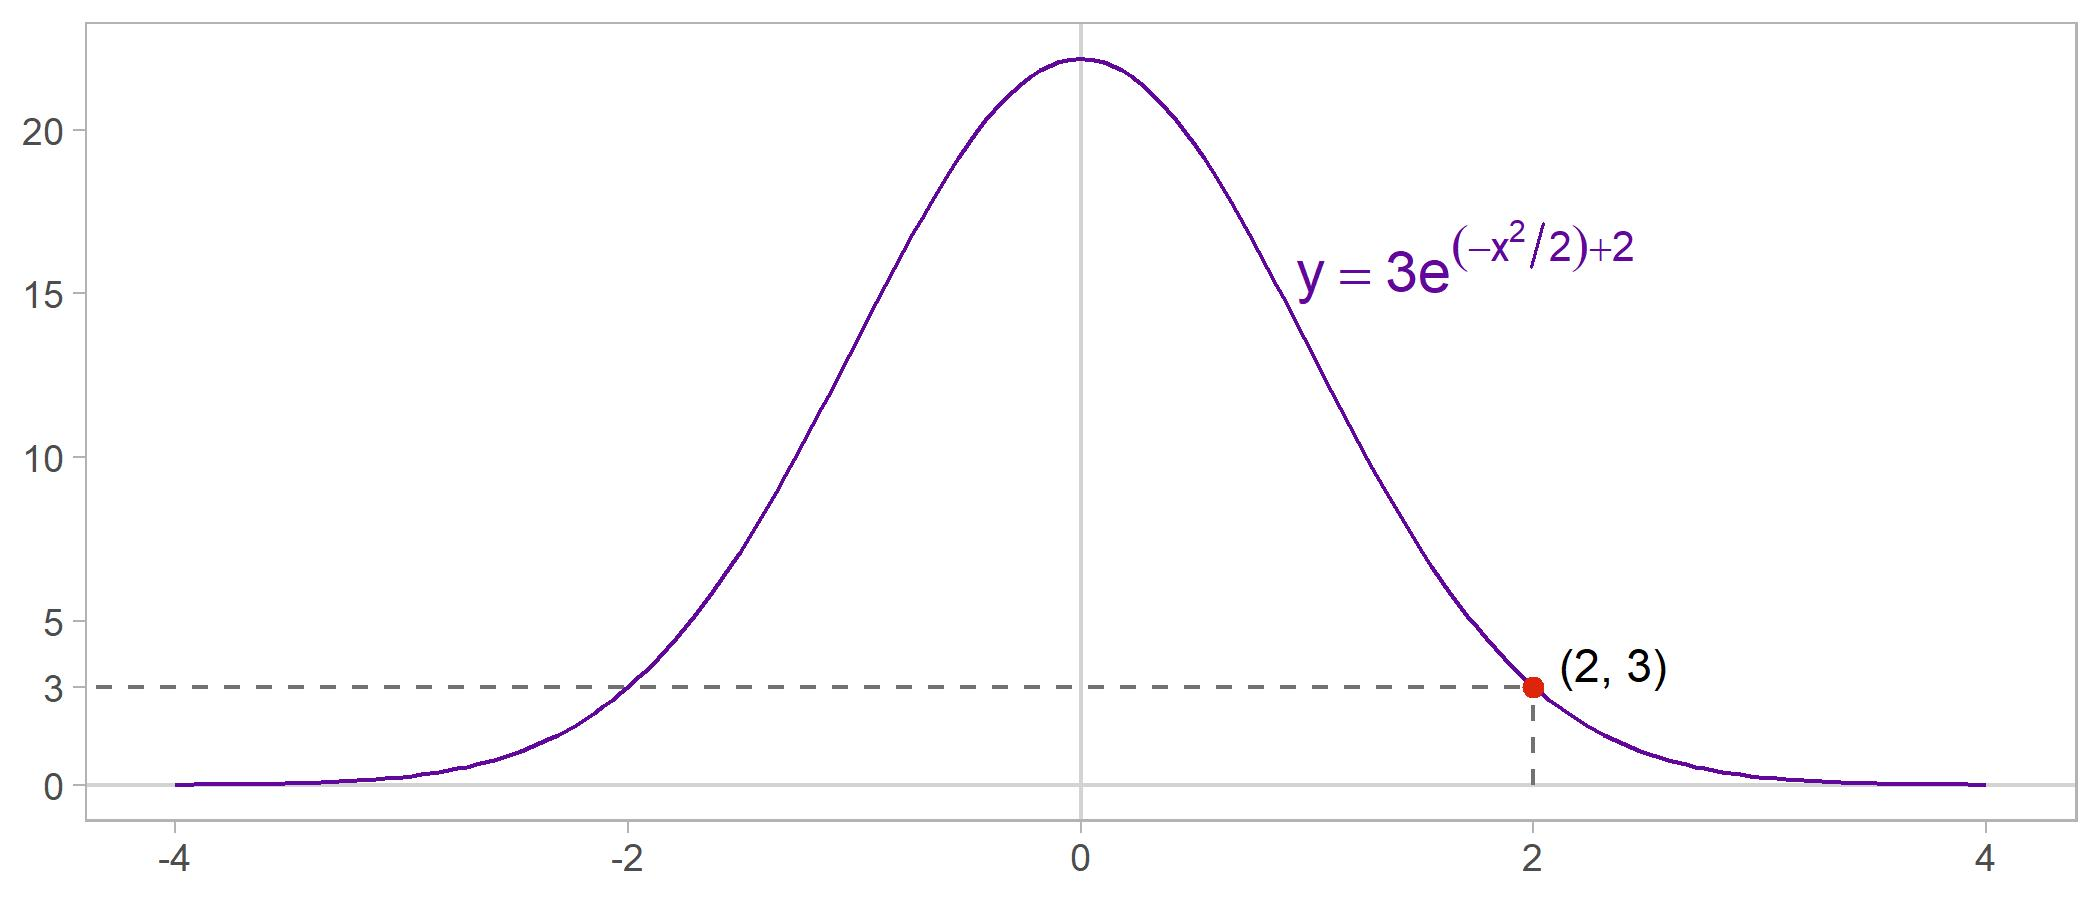
\includegraphics[scale=0.7]{img/diff_eq_exer.jpg}
\end{figure}

\textbf{Ejercicio 2.} \quad Busque un gráfico tal que la pendiente de una línea tangente en $(x, \ y)$ sea el doble de la pendiente de un rayo\footnote{Es una parte de una línea con un punto inicial, pero su punto terminal se ubica en el infinito.} que pasa por los puntos $(0, \ 0)$ y $(x, \ y)$.

\textbf{Solución.} \quad Comencemos calculando la pendiente de este rayo:
\[
  \frac{y - 0}{x - 0} = \frac{y}{x}
\]
Con esto, establezcamos la ecuación diferencial. En el ejercicio nos indican que la pendiente de la línea tangente es el doble de la que corresponde al rayo. Por lo tanto:
\[
  \frac{dy}{dx} = 2 \left(\frac{y}{x}\right)
\]
Luego, apliquemos el método de separación de variables, que es el único que manejamos para resolver este tipo de ecuación.
\begin{align*}
  \frac{dy}{y} &= 2 \left(\frac{dx}{x}\right) \\
  \int \frac{dy}{y} &= 2 \cdot \int \frac{dx}{x} \\
  \ln(\lvert y \rvert) &= 2 \ln(\lvert x \rvert) + C
\end{align*}
En este caso necesitamos que $y$ sea expresada de forma explícita, puesto que buscamos un gráfico para ella. Por lo tanto, debemos calcular la inversa de la última ecuación de arriba.
\begin{align*}
  \exp(\ln(\lvert y \rvert)) &= \exp(2 \ln(\lvert x \rvert) + C) \\
  y &= \exp(C) \cdot \exp(2 \ln(\lvert x \rvert)) \\
  y &= A \cdot (\exp(\ln(\lvert x \rvert)))^{2} \\
  y &= A \cdot x^{2}
\end{align*}
Por lo tanto, la ecuación que nos permite obtener el gráfico que nos piden en el ejercicio, es $y = Ax^{2}$, para todo $\pm A$ y $A = 0$.

Aprovechando, busquemos una función que pase por $(x = 4, \ y = 2)$ y tracemos tanto la línea tangente en dicho punto y el rayo que pase por éste y comience desde el origen.
\begin{align*}
2 &= A (4^{2}) \\
A &= \frac{1}{8} \\
\therefore y &= \frac{1}{8} x^{2}
\end{align*}
Si calculamos la derivada de esta función en $x = 4$, veremos que $y'(4) = 1$ y, en cuanto a la pendiente del rayo, al calcularlo obtenemos que es igual a $(2 - 0)/(4 - 0) = 1/2$. En otras palabras, se cumple que con la familia de funciones que encontramos lo que nos piden. Todo esto lo podemos ver en el siguiente gráfico.

\newpage

\begin{figure}[hbt!]
\centering
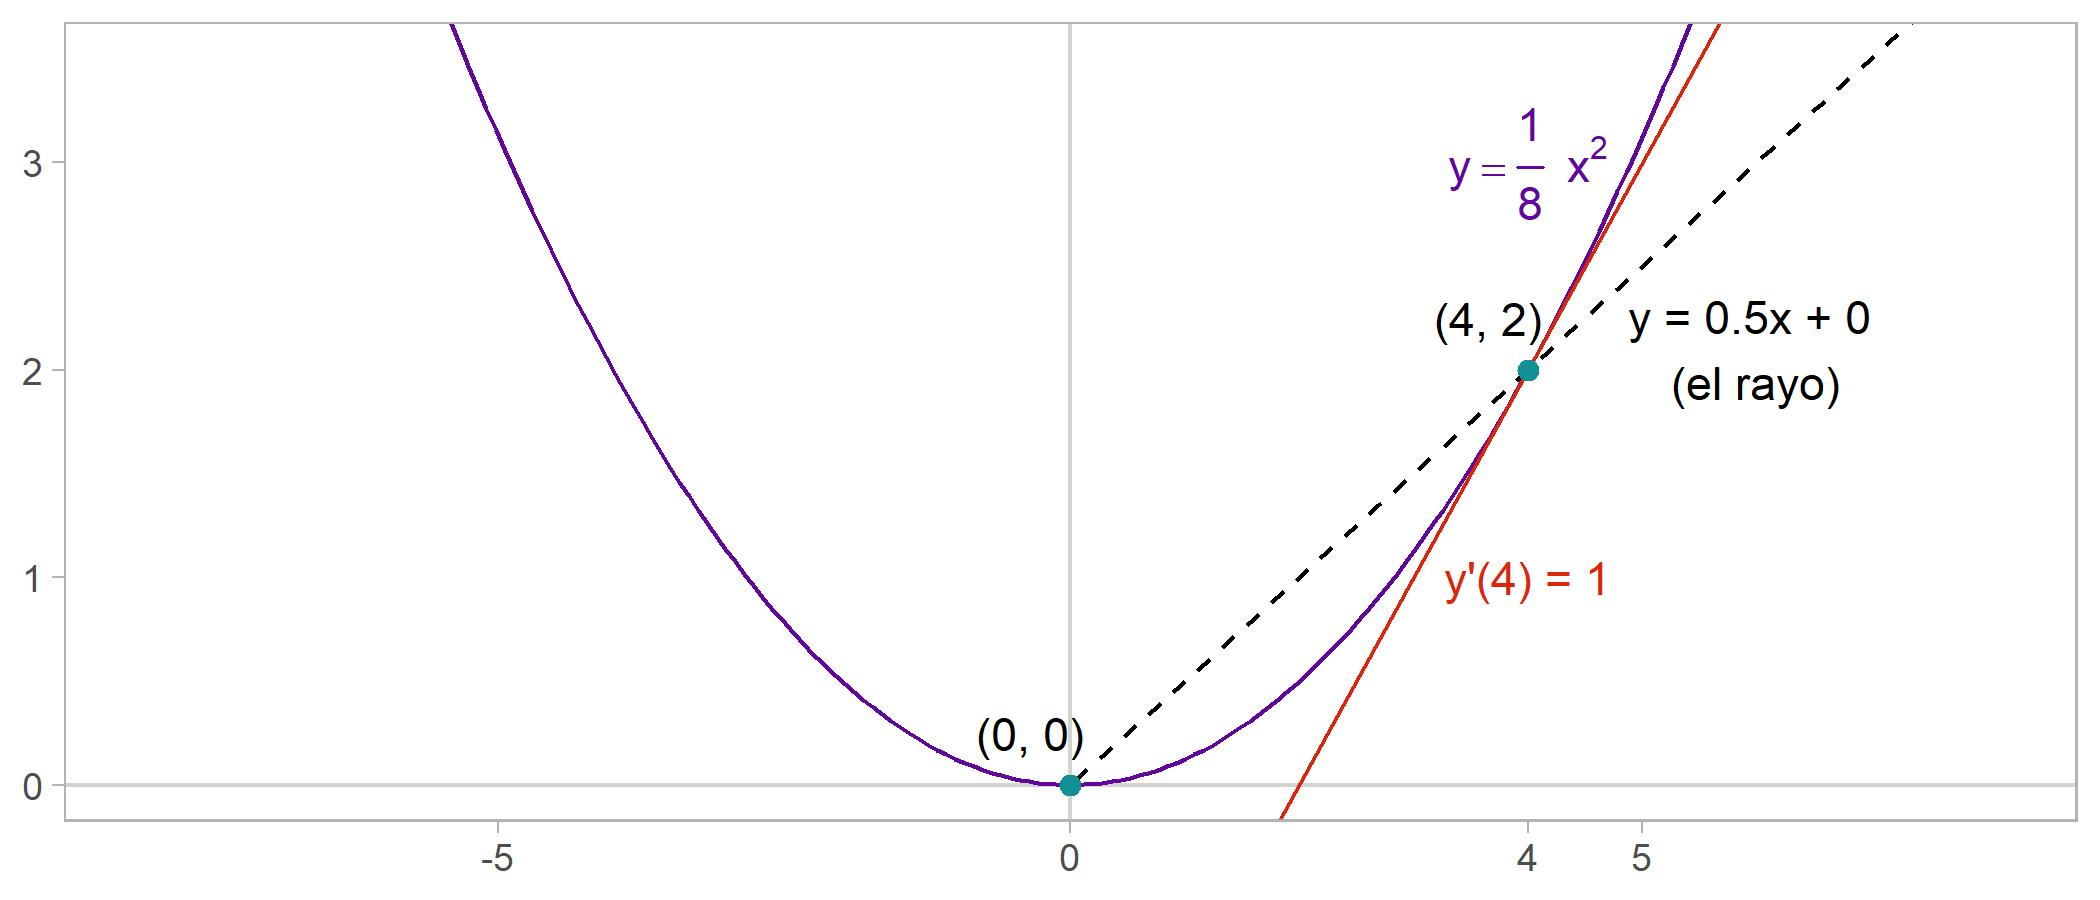
\includegraphics[scale=0.7]{img/diff_eq_exer_2.jpg}
\end{figure}


\subsubsection{Los Campos de Pendientes.}

Es posible conocer el comportamiento de las soluciones de una ecuación diferencial de primer orden, sin tener que resolverla. La herramienta que nos permite aquello, se conoce como \textbf{campo de pendientes}.

El campo de pendientes es una visualización que consiste de pequeños trazos de líneas tangentes, cuyas pendientes están dadas por $dy/dx$ de una ecuación diferencial para cada punto $(x, \ y)$ las que, posteriormente, nos permiten bosquejar curvas sobre ellas, que corresponden a la familia de soluciones de dicha ecuación.

Por ejemplo, a continuación tenemos un campo de pendientes para $dy/dx = x + y$, la cual graficamos usando la calculadora gráfica \textit{online} \href{https://www.desmos.com/calculator/zmpjqh7wl3}{Desmos}.

\begin{figure}[hbt!]
\centering
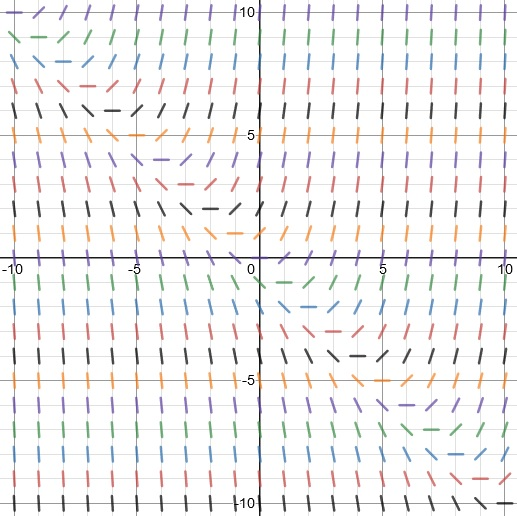
\includegraphics[scale=0.5]{img/slope-field.jpg}
\end{figure}

Como vemos, cada trazo es una línea tangente con pendiente $dy/dx = x + y$, para cada punto del plano.

Además, sin conocer la solución general de $dy/dx = x + y$, podemos trazar una curva que pase por el punto $(0, \ 1)$, dándole su forma a partir de las líneas tangentes. En la siguiente gráfica la dibujamos a mano (color café).

\begin{figure}[hbt!]
\centering
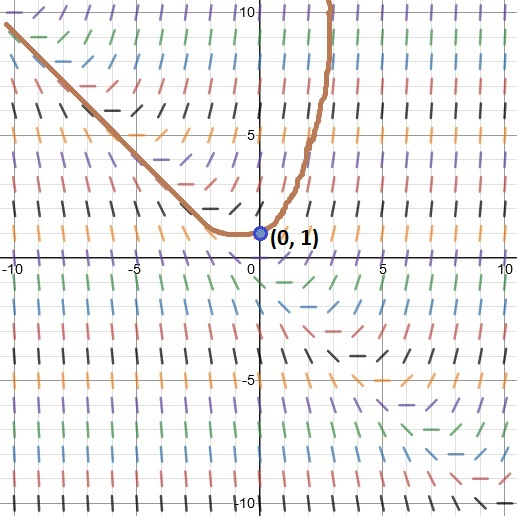
\includegraphics[scale=0.5]{img/slope-field-2.jpg}
\end{figure}

Así, el campo de pendientes podemos entenderlo como una \textbf{solución cualitativa} de una ecuación diferencial, porque nos permite \textbf{tener una idea del comportamiento de su familia de funciones} a partir de la información que ésta nos entregue.

Comprobemos que la curva que trazamos arriba sea una de las soluciones de $dy/dx = x + y$. En este caso no podemos resolverla usando el método de separación de variables, pero usando el software \href{https://www.wolframalpha.com/input/?i=y\%27+\%3D+y+\%2B+x}{WolframAlpha} podemos saber que su solución general es $y = Ae^{x} - x - 1$.

Si establecemos como condición inicial que la función pase por $(0, \ 1)$, entonces:
\begin{align*}
  1 &= Ae^{0} - 0 - 1 \\
  2 &= A \\
  \therefore y &= 2e^{x} - x - 1
\end{align*}
A continuación tenemos su gráfica, también obtenida usando \href{https://www.desmos.com/calculator/byrqbn2so5}{Desmos}.

\newpage

\begin{figure}[hbt!]
\centering
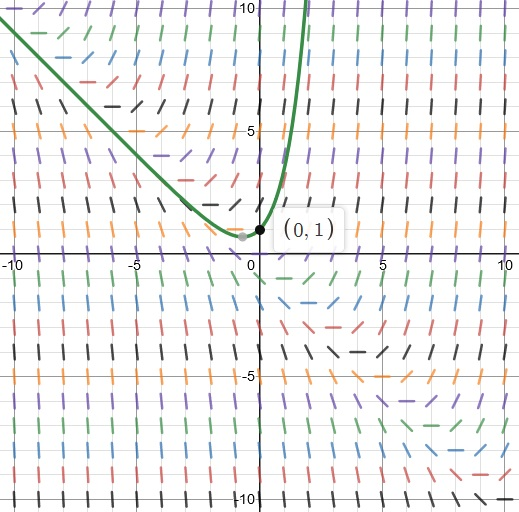
\includegraphics[scale=0.5]{img/slope-field-3.jpg}
\end{figure}

La curva que dibujamos anteriormente es bastante cercana a la real. Esto nos muestra la utilidad que tiene el campo de pendientes para ir teniendo una idea sobre el comportamiento de las curvas de una ecuación diferencial de primer orden.

\subsubsection{Campo de Pendientes y el Método de Euler.}

Al intentar encontrar soluciones de ecuaciones diferenciales, iremos viendo que en varios casos éstas no pueden ser resueltas. Sin embargo, podemos usar el \textbf{Método de Euler} para aproximarnos a ellas.

La idea del método de Euler es \textbf{estimar a una de las funciones de la solución general} calculando \textbf{aproximaciones lineales} para cada punto de ella. Se comienza con el que indica su \textbf{condición inicial} y luego vamos repitiendo el proceso con los puntos finales de cada aproximación lineal. Al unir cada aproximación, veremos que se forma \textbf{una curva} que \textbf{se asimila a una de las funciones de la solución general} de una ecuación diferencial.

Al ser una aproximación lineal, lo ideal es que la distancia entre cada punto desde el inicial en adelante sea lo más corta posible, para tener mayor precisión con respecto a la curva real. No obstante, de igual modo en cierto punto, la tasa de error se irá agrandando.

Sea la siguiente linealización de una función:
\[
  y_{1}(x_{1}) = y_{0}(x_{0}) + y'(x_{0}, \ y_{0}) \Delta x
\]
Donde:

\begin{itemize}
\item Condición inicial $\rightarrow$ $(x_{0}, \ y_{0}(x_{0}))$.
\item Ec. Diferencial en la condición inicial $\rightarrow$ $y'(x_{0}, \ y_{0})$.
\item Punto final de cada aproximación lineal $\rightarrow$ $(x_{1}, \ y_{1})$.
\item Distancia entre cada punto $\rightarrow$ $\Delta x = x_{1} - x_{0}$.
\end{itemize}

Si repetimos este proceso $k$ veces, entonces:
\begin{align*}
  y_{k}(x_{k}) &= y_{k-1}(x_{k-1}) + y'(x_{k-1}, \ y_{k-1}) \Delta x \\
               &= y_{k-1}(x_{k-1}) + y'(x_{k-1}, \ y_{k-1}) (x_{k} - x_{k-1})
\end{align*}
Para visualizar tanto la curva estimada como la real de una de la solución general, podemos usar la siguiente \href{https://mathlets.org/mathlets/eulers-method/}{Mathlet}, desarrollada en el MIT. Las Mathlets son aplicaciones desarrolladas por dicha institución para fines educativos y, una de ellas, sirve para graficar el método de Euler.

Como vemos en el siguiente pantallazo, primero seleccionamos una de las ecuaciones diferenciales disponibles en la aplicación (1); luego elegimos cuál debe ser la distancia entre cada punto o el \textit{stepsize} (2). Posteriormente, clickeamos en cualquier punto en el plano, el cual será nuestra condición inicial (3) y damos click las veces que queramos al botón ``Start'' para que vayan produciéndose las aproximaciones lineales (4). Para compararla con la curva de la solución general, clickeamos donde dice ``Actual'' (5) y luego una vez en ``Start''.

\begin{figure}[hbt!]
\centering
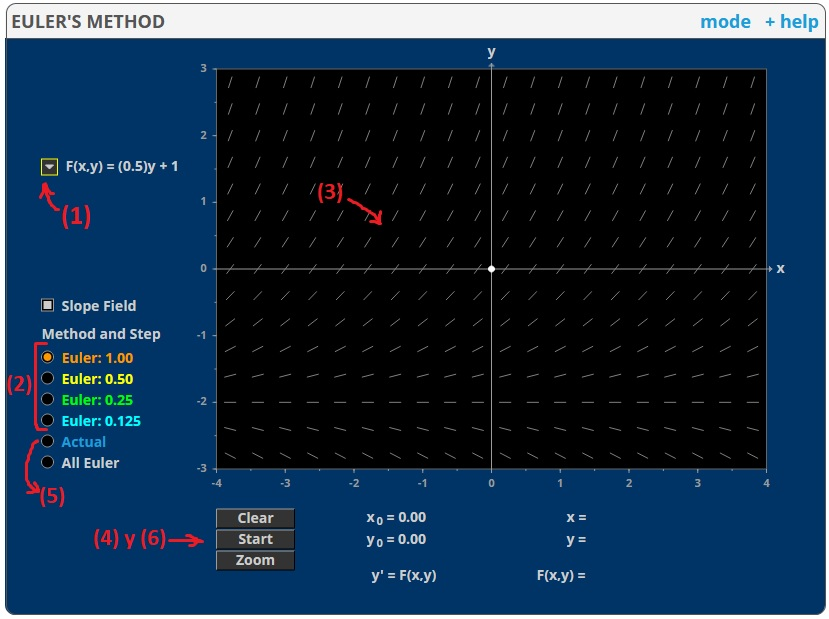
\includegraphics[scale=0.5]{img/screenshot-euler-meth-mathlet.jpg}
\end{figure}


\end{document}
